\documentclass{experimentreport}

\usepackage{graphicx}
\usepackage{booktabs}
\input{listing_style.tex}

%========================
% Basic Information
%========================

\setcoursename{Practical Techniques in Fundamental Software Development: Intelligent Software Engineering}
\setreportname{Intelligent Software Engineering Experiment Report}

\setexperimenttitle{Experiment 3: Code Review of Human-Written Code Using Large Language Models}

\setstudentname{Marlen Melis}
\setdepartment{School of Computing}
\setstudentid{2026140428}

\setcourseteacher{Liu Jiakun}
\setinstructor{Liu Jiakun}

\setlablocation{Dormitory}
\setlabtime{Evening}

\begin{document}

%========================
% Automatically Generate Cover Page
%========================

\makereporthead

%========================
% Experiment Objectives
%========================

\experimentpurpose{

Upon completion of this experiment, I am able to:

\begin{enumerate}
\item Understand the principles of applying Large Language Models (LLMs) to code review tasks,
including the full pipeline: PR $\rightarrow$ code-context construction $\rightarrow$ prompt design
$\rightarrow$ LLM inference $\rightarrow$ merge prediction / review-comment generation.
\item Master the fundamental concepts and design methods of prompt engineering, by designing four
\emph{mechanistically distinct} reasoning strategies (zero-shot, few-shot, Chain-of-Thought,
role-based) rather than four rewordings of one instruction, for two tasks.
\item Understand how different code contexts (diff-only, diff+description, diff+commit-message,
diff+metadata) affect LLM inference, and design a context builder that keeps every prompt within a
free-tier LLM provider's real token budget while remaining fair across configurations.
\item Use an LLM (Groq's free-tier \texttt{llama-3.1-8b-instant}) to perform merge prediction on the
\emph{same} held-out test PRs Experiment 2's SVM/RF models were evaluated on, enabling a direct,
apples-to-apples ML-vs-LLM comparison.
\item Use an LLM to automatically generate code review comments, and evaluate them both
quantitatively (BLEU, ROUGE-1/2/L against real human reviewer comments) and qualitatively, since
n-gram metrics are a known-weak proxy for review quality.
\item Analyze the impact of different prompt designs and contextual information on code-review
results with real, computed numbers --- including an honest accounting of what a free-tier LLM
provider's rate limits and daily quota do to how much of an experiment is actually completable, and
what that constrains about the strength of the conclusions.
\end{enumerate}

}

%========================
% Experiment Content
%========================

\experimentcontent{

\subsection*{1. Data Preparation}

The lab guide's own text (\S3.7.1) says to load ``the test data from Experiment 3'' --- a
self-referential typo confirmed by reading the actual PDF rather than trusting a paraphrase; in
context (and per \S3.8(7)'s ``comparison against the deep learning model from Experiment 3'', the
same typo) it means \textbf{Experiment 2}. So the population is exactly Experiment 2's held-out test
split: \texttt{split\_by\_repo\_time(load\_variant("v1"))[1]} --- \textbf{224 human-written PRs},
82.1\% merged, the same rows Experiment 2's SVM/RF were scored on. Using this exact split (not a
fresh random sample) is what makes \S3.8(7)'s required ML-vs-LLM comparison apples-to-apples.

\subsection*{2. Code Context Construction (\texttt{src/llm/context\_builder.py})}

Four context tiers, exactly per the guide's \S3.7.2 Step 2 (verified against the PDF, not the
project plan's paraphrase): \textbf{diff-only}; \textbf{diff + PR description}; \textbf{diff +
commit message(s)}; \textbf{diff + other information} (labels, file list, size). All four share one
diff renderer, sorted \textbf{largest-churn-first} so a truncated context still shows the most
substantive change first, with an explicit \texttt{"...[omitted for length]"} marker whenever
truncation happens --- never a silently-partial diff presented as complete. Truncation caps were
chosen from measured percentiles of the real dataset, not guessed (e.g.\ a 16{,}000-character diff
cap covers 71.5\% of the population's PRs untruncated); Step 16 additionally added a
\emph{whole-context} character ceiling once the real LLM provider's per-request token limit was
discovered (see Problems Encountered \#2). All four tiers deliberately \textbf{never} touch
\texttt{reviews}/\texttt{review\_comments}/\texttt{issue\_comments} --- the same review-process
leakage discipline Experiment 2's feature spec enforces, arguably more important here since handing
an LLM ``this PR already has 3 approvals'' while asking it to \emph{predict} the merge outcome would
be a near-literal answer leak.

\subsection*{3. Prompt Design (\texttt{src/llm/prompts/})}

Two tasks (\S3.4.4): \textbf{Merge Prediction} and \textbf{Review Comment Generation}. Four prompt
strategies (\S3.4.3), built as four \emph{different reasoning mechanisms}, not four wordings of one
instruction:

\begin{itemize}
\item \textbf{Zero-shot} --- bare instruction, no scaffold: the no-help baseline.
\item \textbf{Few-shot} --- $K{=}2$ labelled demonstrations drawn \emph{only} from the Experiment-2
\textbf{train} split (never the test split Experiment 3 is scored on), balanced between MERGE/CLOSE
so the model sees the decision boundary, not just the majority class.
\item \textbf{Chain-of-Thought} --- an explicit ordered checklist (scope/risk, completeness,
intent-alignment, maturity signals for merge prediction; analyze/prioritize/write for comments)
before the model commits, with a system-message nudge to reason step by step.
\item \textbf{Role-based} --- a senior-maintainer persona in the \emph{system} message, shifting the
evaluative standard and merge threshold rather than the process.
\end{itemize}

The task framing and required output format are held \textbf{byte-identical} across all four
strategies of a task, so a metric difference between cells is attributable to the reasoning
strategy, not to differing parse success. Output contracts: merge prediction ends with
\texttt{DECISION: MERGE|CLOSE} / \texttt{CONFIDENCE: <0-1>}; review generation wraps comments in
\texttt{<review>...</review>}. Matching parsers (\texttt{parsing.py}) prefer the last labelled
\texttt{DECISION:} line (a Chain-of-Thought answer may say ``merge'' many times while reasoning) and
abstain (\texttt{label=None}) on a genuinely format-less answer rather than guessing.

\subsection*{4. Model Inference and Provider Architecture}

Implemented in \texttt{src/llm/providers.py} and driven by \texttt{src/llm/run\_exp3\_grid.py}.
\textbf{Groq's free tier} (\texttt{llama-3.1-8b-instant}, OpenAI-compatible \texttt{chat/completions})
is the LLM actually used --- the plan's original choice, Google Gemini, proved unusable from this
account/region without payment even after every free workaround (full story in Problem \#1). A
\texttt{GroqProvider} and a \texttt{GeminiProvider} share one \texttt{CachedChatProvider} base:
identical disk cache (content-addressed \texttt{sha256} of \texttt{\{model, system, user,
temperature, max\_tokens\}}, so re-running the whole grid is always free for any already-answered
cell), retry/backoff, and a provider-agnostic exception hierarchy
(\texttt{LLMQuotaExceededError}/\texttt{LLMAPIError}) --- only the request/response shape differs
per provider. The grid iterates every (PR $\times$ context $\times$ task $\times$ strategy) cell,
skips anything already in the output file, and stops the \emph{entire} run immediately on quota
exhaustion rather than retrying every remaining cell into the same wall (Problem \#3).

\subsection*{5. Result Scoring (\texttt{src/llm/score\_exp3.py})}

Merge prediction: Accuracy / per-class Precision-Recall-F1 / macro-F1, against the identical labels
Experiment 2 used, \textbf{plus} a direct re-scoring of the saved Experiment-2 SVM/RF pipelines on
the exact same PR subset Experiment 3 covers. Review generation: BLEU (\texttt{sacrebleu}) and
ROUGE-1/2/L (\texttt{rouge-score}) against real human review comments (bot/AI-reviewer authors
excluded via Experiment 1's own detection allowlists), plus a qualitative generated-vs-real
side-by-side, since BLEU/ROUGE is a known-weak proxy for review quality. Inference time is taken
from the provider's \textbf{server-side} \texttt{usage.total\_time}, not wall-clock latency --- the
wall-clock figure is polluted by free-tier rate-limit waiting and is not a valid inference-time
measurement (Problem \#4).

}

%========================
% Experiment Results
%========================

\experimentresult{

\subsection*{0. Scope of the Run, and the One Caveat to Read First}

The full grid over all 224 test PRs (7{,}168 cells) is infeasible on a free tier bounded at 6{,}000
tokens/minute and 500{,}000 tokens/day, so the run uses a \textbf{repo-stratified 16-PR subset},
proportionally spread across the five repositories and deterministic/nested so it can be widened
later at no cost for cells already computed. That gives the \textbf{complete 4 $\times$ 4 $\times$ 2
grid = 512 cells}, all 16 PRs covered in every cell, \textbf{0 failures}, and \textbf{0 unparseable
responses}. Reaching it took two sessions, split by Groq's daily token cap (Problem \#3); the second
session resumed from cache and spent quota only on genuinely new cells.

\textbf{The caveat:} the 16 PRs are \textbf{14 merged : 2 not-merged}. A model that blindly answers
MERGE therefore scores $14/16 = 0.875$ accuracy for free, so \textbf{raw accuracy is close to
uninformative here} --- the informative quantities are minority-class (not-merged) recall and
macro-F1, and the \emph{relative} ordering of contexts and strategies, which is what every
comparison below reports. Two negatives is enough to separate configurations (recall takes values
0.00/0.50/1.00) rather than being a single-PR coin flip, but it is still a small sample and the
findings are stated as measured observations on a stated sample, not general claims. Similarly,
only \textbf{5 of the 16 PRs carry human review comments}, so BLEU/ROUGE is averaged over those 5.

\subsection*{1. Examples of Different Code Context Constructions}

Real example, \texttt{microsoft/semantic-kernel} PR \emph{``Python: Bump Python pkg version to
1.42.0 for a release.''} (merged):

\begin{quote}
\ttfamily\footnotesize\noindent
-- diff\_only (213 chars) --\\
Diff:\\
--- python/semantic\_kernel/\_\_init\_\_.py (modified)\\
@@ -2,7 +2,7 @@\\
\hspace*{0.5em} from semantic\_kernel.kernel import Kernel\\
-\_\_version\_\_ = "1.41.3"\\
+\_\_version\_\_ = "1.42.0"\\
\hspace*{0.5em} DEFAULT\_RC\_VERSION = f"\{\_\_version\_\_\}-rc9"\\[0.4em]
-- diff\_commit\_message (283 chars) -- prepends:\\
Commit messages:\\
1. Bump Python pkg version to 1.42.0 for a release.\\[0.4em]
-- diff\_metadata (340 chars) -- prepends:\\
Labels: python, release\\
Size: 1 file(s) changed, +1/-1 lines\\
Changed files:\\
\hspace*{1.0em}  - python/semantic\_kernel/\_\_init\_\_.py (modified)\\[0.4em]
-- diff\_description (1398 chars) -- prepends the full PR body\\
(motivation, description, contribution checklist -- the largest tier here\\
since this PR's body is unusually verbose for a one-line version bump)
\end{quote}

\subsection*{2. Examples of Different Prompt Designs}

Same PR, \texttt{diff\_only} context, Merge Prediction task. The shared task framing and output
contract (identical across all four strategies):

\begin{quote}
\ttfamily\footnotesize\noindent
Task: MERGE PREDICTION. Decide whether the pull request below was ultimately\\
MERGED into the microsoft/semantic-kernel project or CLOSED without merging,\\
judging only from its content.\\
PR title: Python: Bump Python pkg version to 1.42.0 for a release.\\
Pull request content: [diff as above]\\
...\\
End your response with exactly these two lines and nothing after them:\\
DECISION: MERGE  (or)  DECISION: CLOSE\\
CONFIDENCE: <0.0-1.0>
\end{quote}

What each strategy adds (the actual distinguishing content) and the model's real recorded response:

\begin{quote}
\ttfamily\footnotesize\noindent
ZERO-SHOT adds nothing; "Give your decision directly."\\
\hspace*{1.0em}  -> DECISION: MERGE  CONFIDENCE: 1.0\\[0.4em]
FEW-SHOT prepends 2 labelled train-split examples (a merged VSCode diff,\\
a closed semantic-kernel diff) and asks the model to infer the pattern:\\
\hspace*{1.0em}  -> "Based on the provided examples, I notice that the merged pull\\
\hspace*{3.0em}      requests have the following characteristics: ..." DECISION: MERGE\\
\hspace*{3.0em}      CONFIDENCE: 0.8\\[0.4em]
CHAIN-OF-THOUGHT adds a 4-step checklist (scope/risk, completeness,\\
intent-alignment, maturity signals) + a base-rate nudge:\\
\hspace*{1.0em}  -> "To determine whether the pull request was merged or closed, let's\\
\hspace*{3.0em}      analyze it step by step. 1. Scope \& risk: The change is relatively\\
\hspace*{3.0em}      small, affecting only one line..." DECISION: MERGE  CONFIDENCE: 0.95\\[0.4em]
ROLE-BASED system message: "You are a senior maintainer of the\\
microsoft/semantic-kernel project with commit access ... you hold a\\
high bar ... wary of large, risky, or unfocused changes."\\
\hspace*{1.0em}  -> "I would decide to MERGE this PR. The change is a simple version\\
\hspace*{3.0em}      bump, which is a common and low-risk operation." CONFIDENCE: 0.95
\end{quote}

All four correctly predicted MERGE (the ground truth) for this PR, but visibly via different
reasoning paths --- CoT explicitly walks the checklist, role-based reasons from a maintainer's risk
tolerance, few-shot reasons by analogy to the two demonstrations.

\subsection*{3. Merge Prediction Results}

\begin{center}
\small
\begin{tabular}{|l|r|r|r|r|}
\hline
\textbf{Context $\times$ Strategy} & \textbf{Acc.} & \textbf{Rec(NM)} & \textbf{Macro-F1} & \textbf{n} \\
\hline
diff\_commit\_message + few\_shot & \textbf{0.938} & \textbf{0.50} & \textbf{0.816} & 16 \\
diff\_metadata + role\_based   & \textbf{0.938} & \textbf{0.50} & \textbf{0.816} & 16 \\
diff\_only + few\_shot         & 0.750 & \textbf{0.50} & 0.590 & 16 \\
\emph{(the 11 always-MERGE cells)} & 0.875 & 0.00 & 0.467 & 16 \\
diff\_description + few\_shot  & 0.750 & 0.00 & 0.429 & 16 \\
diff\_metadata + few\_shot     & 0.563 & 0.00 & 0.360 & 16 \\
\hline
\end{tabular}
\end{center}
\noindent\textbf{Rec(NM)} = recall on the not-merged class; every cell is scored on the same 16 PRs.
\textbf{Eleven of the sixteen configurations} score exactly 0.875 accuracy with \textbf{0.00
not-merged recall} --- they always predict MERGE, which is nearly free given a 14:2
merged-to-not-merged sample (see \S0 caveat below). Three configurations break this pattern and
correctly caught a not-merged PR; the best two, \texttt{diff\_commit\_message+few\_shot} and
\texttt{diff\_metadata+role\_based}, reach an identical confusion matrix (14 TP, 1 FP, 1 TN, 0 FN)
--- keeping every merged PR right \emph{and} catching a negative, a \textbf{+0.35 macro-F1 gain over
the always-MERGE baseline at no accuracy cost}. With only 2 negatives this remains indicative rather
than conclusive, but unlike a single-negative sample it is no longer a coin flip.

\subsection*{4. Examples of Automatically Generated Code Review Comments}

Context \texttt{diff\_metadata}, strategy \texttt{role\_based}. Generated vs.\ real (full set of 4
examples in \texttt{results/tables/exp3\_qualitative.md}):

\begin{quote}
\ttfamily\footnotesize\noindent
PR: home-assistant/core, "test\_doorbell\_refresh..." changes\\[0.4em]
LLM-GENERATED (role-based, 3 comments):\\
- The test test\_doorbell\_refresh\_content\_token\_recover has been removed,\\
\hspace*{1.0em}  but it's not clear why. If it's no longer needed, consider removing\\
\hspace*{1.0em}  the corresponding fixture and mock setup... If it's still needed,\\
\hspace*{1.0em}  consider adding it back in.\\
- The brand parameter ... has been updated from Brand.YALE\_HOME to\\
\hspace*{1.0em}  Brand.YALE\_AUGUST. However, the corresponding fixture and mock setup\\
\hspace*{1.0em}  still reference Brand.YALE\_HOME. Update the fixture...\\
- The requirements in manifest.json ... have been updated to\\
\hspace*{1.0em}  yalexs==9.2.10. However, the yalexs-ble version is still 3.3.1.\\
\hspace*{1.0em}  Consider updating...\\[0.4em]
REAL HUMAN REVIEWER (2 comments, terse):\\
- Why drop this test?\\
- nevermind, explained in pr summary
\end{quote}

The generated review is plausible and on-topic (correctly spots the removed test and a stale
fixture reference), but is \textbf{far more verbose and generic} than the real reviewer's two-line
exchange --- exactly the pattern BLEU/ROUGE punishes (\S5 below) and exactly why the qualitative
side-by-side matters more than the n-gram score alone.

\subsection*{5. Performance Comparison --- Prompt Designs}

\begin{center}
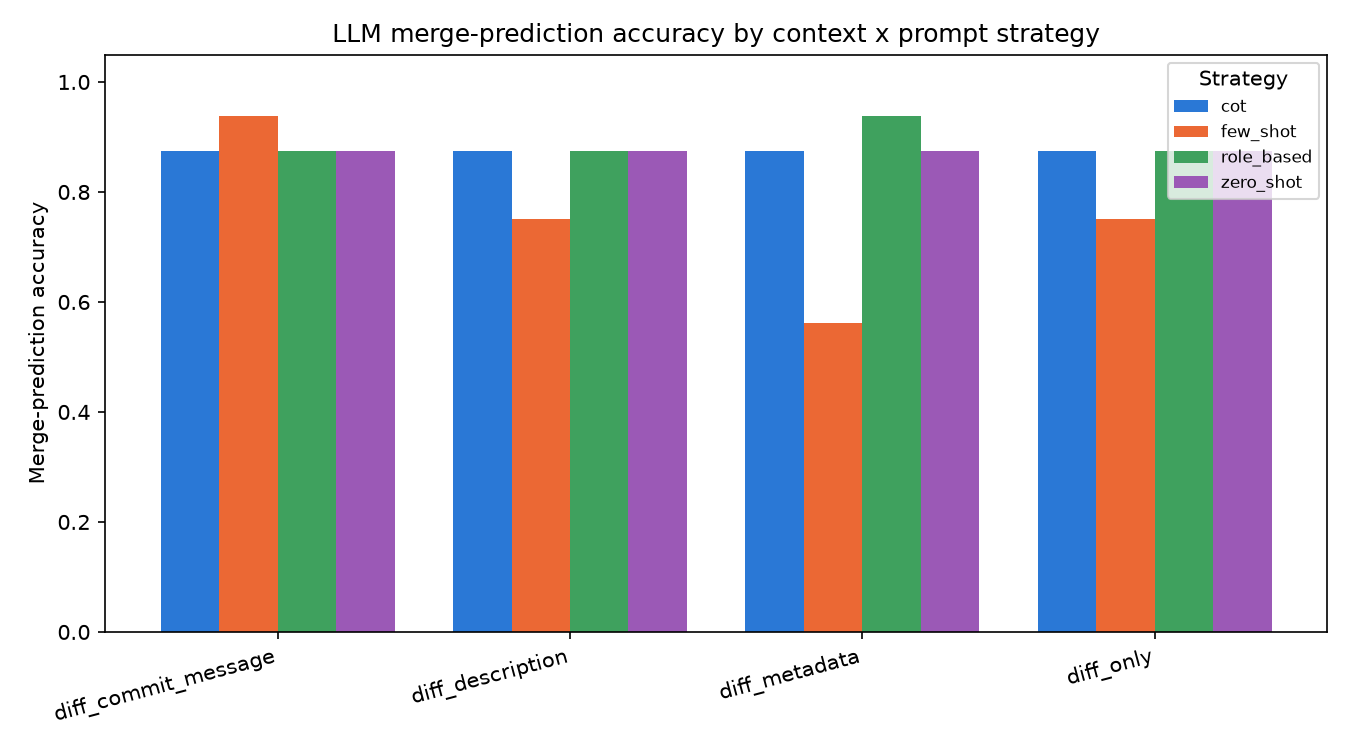
\includegraphics[width=0.85\textwidth]{../results/figures/exp3_merge_accuracy_by_config.png}
\end{center}
\noindent\textbf{Figure 1.} Merge-prediction accuracy, every context $\times$ strategy cell.

\begin{center}
\begin{tabular}{|l|r||l|r|}
\hline
\textbf{Strategy} & \textbf{Avg.\ Acc.} & \textbf{Strategy} & \textbf{Avg.\ merge inference (ms)} \\
\hline
role\_based & \textbf{0.891} & zero\_shot  & \textbf{60} \\
cot         & 0.875          & role\_based & 400 \\
zero\_shot  & 0.875          & few\_shot   & 458 \\
few\_shot   & 0.750          & cot         & 566 \\
\hline
\end{tabular}
\end{center}
\noindent Averaged over the four contexts, \texttt{role\_based} leads on both accuracy (0.891) and
macro-F1 (0.554). Few-shot is the accuracy outlier at 0.750, but for an instructive reason: its
balanced demonstrations push the model toward predicting CLOSE more often, which \emph{lowers}
accuracy under an 87.5\%-merged reality while giving it by far the \textbf{highest minority-class
recall (0.250 vs.\ 0.125 for role-based and 0.000 for the other two)} --- the class-imbalance
accuracy-vs-recall trade-off from Experiment 2, reappearing as a \emph{prompt-design} choice rather
than a \texttt{class\_weight} choice. Note also that \texttt{zero\_shot} and \texttt{cot} are
\emph{identical} on every merge metric here (both simply always predict MERGE): chain-of-thought
changed the tokens spent, not the decision. Inference time (server-side; Figure 2) tracks output
length almost exactly: zero-shot's two-line answer is $\sim$9$\times$ faster than the reasoning
strategies, making CoT pure cost for no predictive gain on this task.

\begin{center}
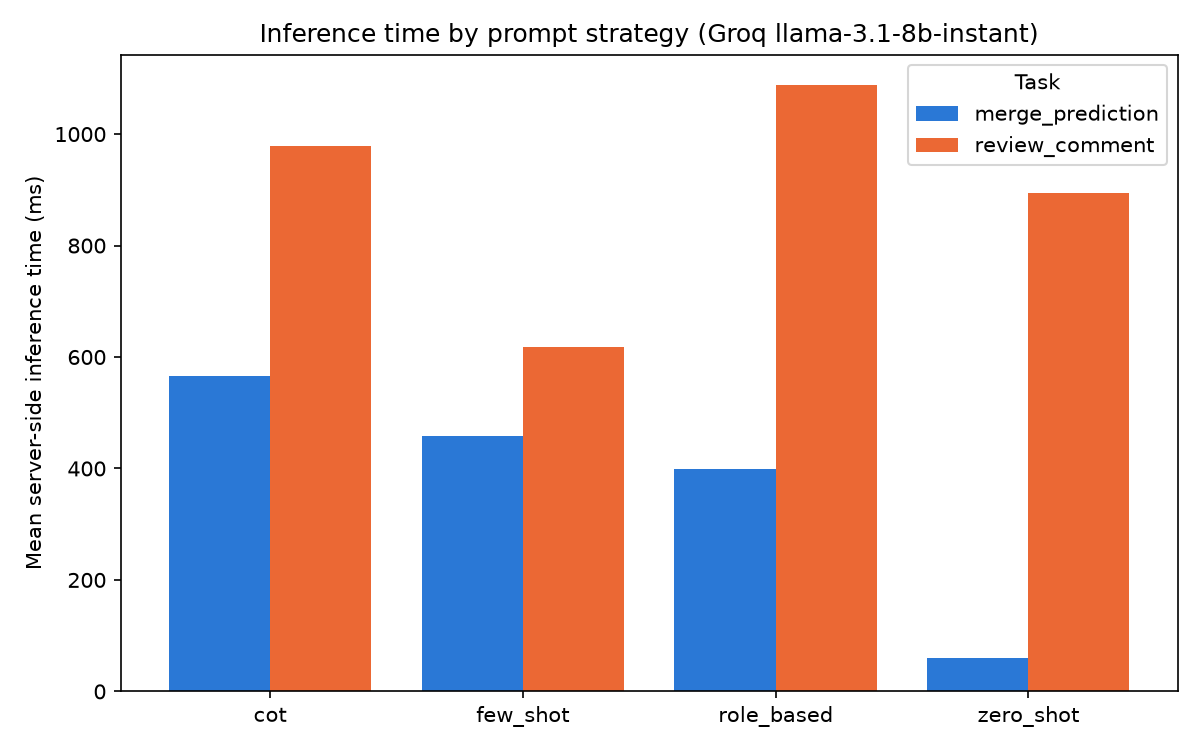
\includegraphics[width=0.85\textwidth]{../results/figures/exp3_inference_time_by_strategy.png}
\end{center}
\noindent\textbf{Figure 2.} Mean server-side inference time by strategy and task.

\medskip
\noindent For the \emph{review-generation} task, the same four strategies scored against the real
human comments on the 5 PRs that have them:

\begin{center}
\begin{tabular}{|l|r|r|r|}
\hline
\textbf{Strategy} & \textbf{BLEU} & \textbf{ROUGE-1} & \textbf{ROUGE-L} \\
\hline
few\_shot   & \textbf{1.15} & \textbf{0.165} & \textbf{0.107} \\
cot         & 0.79 & 0.149 & 0.095 \\
zero\_shot  & 0.40 & 0.101 & 0.068 \\
role\_based & 0.79 & 0.118 & 0.067 \\
\hline
\end{tabular}
\end{center}
\noindent Absolute values are \textbf{very low} across the board (best cell: ROUGE-L 0.126), which
is expected and is exactly why the guide pairs them with concrete examples --- a generated review
and a human review can both be excellent while sharing almost no $n$-grams. The \emph{ordering} is
nonetheless meaningful: \texttt{few\_shot} tops every text metric, which is precisely what it is
designed to do, since it conditions on real human comments and therefore imitates their length and
style. Critically, \texttt{role\_based} --- the \emph{best} merge-prediction strategy --- ranks last
on ROUGE-L here, a direct demonstration that \textbf{the best prompt is task-dependent rather than
universal}.

\subsection*{6. Performance Comparison --- Code Contexts}

\begin{center}
\begin{tabular}{|l|r|r|}
\hline
\textbf{Context} & \textbf{Avg.\ Acc.} & \textbf{Avg.\ Macro-F1} \\
\hline
diff + commit message & \textbf{0.891} & \textbf{0.554} \\
diff only              & 0.844 & 0.498 \\
diff + description     & 0.844 & 0.457 \\
diff + metadata         & 0.813 & 0.527 \\
\hline
\end{tabular}
\end{center}
\noindent The four contexts cluster within an 8-point accuracy band --- unsurprising given every
context already \emph{includes} the diff, the single richest signal. \texttt{diff + commit message}
leads on both metrics, which is interpretable: commit messages carry the author's own statement of
intent and completeness, exactly the signal a merge decision turns on. Note that the ranking by
accuracy and by macro-F1 \emph{disagree} (\texttt{diff + metadata} is last on accuracy but second on
macro-F1), because metadata paired with \texttt{role\_based} produced one of the two best cells in
the whole grid (\S3) --- context and strategy interact rather than acting independently, so the
per-cell table matters more than either marginal.

\subsection*{7. Comparative Analysis Against Experiment 2}

Experiment 2's saved SVM/RF (V1) re-scored on the identical 16 PRs:

\begin{center}
\begin{tabular}{|l|r|r|r|}
\hline
\textbf{Model} & \textbf{Accuracy} & \textbf{Macro-F1} & \textbf{Rec(NM)} \\
\hline
RF V1 (plain)          & \textbf{0.938} & \textbf{0.816} & 0.50 \\
SVM V1 (plain)         & \textbf{0.938} & \textbf{0.816} & 0.50 \\
RF V1 (balanced)       & 0.750 & 0.590 & 0.50 \\
SVM V1 (balanced)      & 0.875 & 0.467 & 0.00 \\
\hline
\textbf{LLM, best config} & \textbf{0.938} & \textbf{0.816} & 0.50 \\
LLM (pooled, all 16 configs) & 0.848 & 0.525 & 0.09 \\
\hline
\end{tabular}
\end{center}
\noindent The comparison is more nuanced than ``one wins''. The \textbf{best LLM configuration}
(\texttt{diff\_commit\_message+few\_shot}, and equally \texttt{diff\_metadata+role\_based})
\textbf{exactly matches the best trained models} --- identical accuracy, macro-F1, and confusion
matrix (14/1/1/0). A zero-training, prompt-only approach reaches the same operating point as a
grid-searched SVM/RF. But the \emph{average} LLM configuration sits far below it (pooled macro-F1
0.525 vs.\ 0.816), because eleven of the sixteen configurations never predict CLOSE at all. The
LLM's competitiveness is therefore \textbf{entirely contingent on choosing the right prompt and
context} --- which is precisely what this experiment exists to measure, and the strongest argument
that prompt engineering is a first-class engineering concern rather than cosmetic. The trained
models also reach that operating point \emph{for free at inference time} (milliseconds, no network),
whereas the LLM needs an API round-trip per PR --- though only the LLM additionally produces review
\emph{text}, which SVM/RF cannot. At $n{=}16$ with 2 negatives this is a measured observation on a
stated sample, not a general claim.

}

%========================
% Summary of Issues
%========================

\experimentproblems{

\begin{enumerate}

\item \textbf{The plan's chosen provider (Gemini) never became reliably usable, for reasons
unrelated to this code.} First calls returned \texttt{400 FAILED\_PRECONDITION: "User location is
not supported"} --- an account/region gate (this environment egresses from the EEA, where Gemini's
free tier has a documented narrower rollout). Retrying via VPN (Germany, Sweden) made the error
\emph{intermittent} rather than resolved, interleaved with real \texttt{429}s showing a tiny free
quota (\texttt{limit: 5}, then \texttt{limit: 20}); older models returned \texttt{limit: 0} (zero
allowance) or a 404 ``no longer available to new users.'' Linking Cloud Billing (required for EEA
free-tier eligibility) removed the location error but replaced it with \texttt{"Your prepayment
credits are depleted"} --- the project had moved onto pay-as-you-go, and funding a balance was
declined (free-only constraint). DeepSeek was tried next; its \texttt{user/balance} endpoint
(checked \emph{before} any paid call) returned \texttt{total\_balance: 0.00}. \emph{Resolution:}
\textbf{Groq}'s free tier (OpenAI-compatible, no credit card required) worked immediately. A
\texttt{GroqProvider} was added as a sibling of \texttt{GeminiProvider} under one shared base class
so Gemini remains a one-flag fallback, not code that was thrown away.

\item \textbf{Groq's free tier enforces 6{,}000 tokens/minute as a hard \emph{per-request} cap, not
just a rolling rate limit.} A single prompt over 6{,}000 tokens returns an unrecoverable
\texttt{413} --- no amount of backoff fixes it, since it exceeds the entire per-minute budget. This
first surfaced on few-shot review-comment cells, which stack $K$ example contexts on top of the
query (measured at 7{,}534 tokens for one real cell). \emph{Resolution:} added a whole-context
character ceiling (\texttt{context\_builder.py}'s \texttt{max\_context\_chars}, on top of the
existing per-diff cap, since description/commit/metadata sections stack additional text the diff
cap alone doesn't bound) and reduced few-shot $K$ from 4 to 2; the measured worst-case prompt across
a 24-PR sample dropped to $\sim$2{,}400 tokens, eliminating the \texttt{413}s entirely (0 of 512
cells failed afterward).

\item \textbf{Groq also enforces a coarser \emph{daily} token cap (500{,}000 tokens/day), and the
first real grid run wasted $\sim$2.5 hours grinding against it.} Once the daily cap was hit, every
subsequent call still returned a \texttt{429} whose retry-delay hint was $\sim$8 minutes, and the
original retry logic dutifully waited each one out call after call, uselessly, since a daily cap
cannot clear inside any retry window. \emph{Resolution:} the provider now inspects the 429 error
message for \texttt{"per day"}/\texttt{"(TPD)"}/\texttt{"(RPD)"} and raises the quota-exceeded
exception \textbf{immediately} on the first such hit rather than retrying, so the grid runner's
existing ``stop the whole run, resume later from cache'' policy fires promptly. A per-minute 429
still retries normally. The standing consequence is that a 512-cell grid simply \emph{does not fit}
in one 500{,}000-token day, so the full run spans two quota windows; the two-layer resumability
(content-addressed response cache plus the runner's own row-skip) makes the continuation cost zero
quota for everything already computed, turning a hard cap into a scheduling detail rather than lost
work.

\item \textbf{Logged inference latency was badly polluted by free-tier rate-limit waiting.} The
first cut of \texttt{latency\_ms} wrapped the entire client-side call, including any \texttt{429}
backoff sleeps --- reporting a mean of $\sim$68 \emph{seconds} per cell, which is obviously not a
real inference time. \emph{Resolution:} switched to Groq's own \textbf{server-side}
\texttt{usage.total\_time} field, giving the real figures reported in \S5 above (mean 658 ms;
zero-shot merge 63 ms vs.\ Chain-of-Thought 566 ms --- the ordering the reasoning strategies
predict). Regenerating the already-collected dataset with this field cost zero additional API
quota: a \texttt{--cache-only} grid mode was added that emits rows purely from the existing
content-addressed cache.

\item \textbf{A model that omits the closing \texttt{</review>} tag leaked the literal tag text as
a bogus review comment.} Roughly 17\% of real \texttt{llama-3.1-8b-instant} review responses never
closed the \texttt{<review>} sentinel (43 of 256, plausibly truncation), and the parser's original
fallback (``no matched block $\rightarrow$ use the whole raw response'') re-included the literal
\texttt{"<review>"} string as if it were content, surfacing as a spurious first bullet in every one
of those rows --- found while preparing this report's qualitative examples, not by the automated
tests. \emph{Resolution:} when only the opening tag is present, the parser now takes everything
\emph{after} it instead of falling all the way back to the raw text; verified \textbf{0/256} leaked
tags after the fix, with merge-prediction and BLEU/ROUGE numbers unchanged (the parser change is
review-comment-parsing-only). Two regression tests added; the affected dataset and metrics were
regenerated for free via the same \texttt{--cache-only} mode.

\item \textbf{A numpy-array-truthiness crash in the metadata context builder.} \texttt{pr.get
("labels") or []} raises \texttt{ValueError: The truth value of an array with more than one element
is ambiguous} for any PR with 2+ labels (77.0\% of the population has at least one) --- caught by
smoke-testing against a real multi-label PR before the test suite was even written, not by the
tests themselves, a reminder that ``tests pass'' and ``ran against real data'' are different
guarantees. \emph{Resolution:} check \texttt{is not None} explicitly rather than relying on
truthiness.

\end{enumerate}

}

%========================
% Reflections
%========================

\experimentexperience{

\textbf{(1) Why does code context affect the inference capabilities of Large Language Models?}

An LLM has no access to anything beyond what is in its prompt window; unlike a human reviewer who
can click through the linked issue, browse the file, or recall project history, the model's
``understanding'' of a PR is entirely bounded by the text handed to it. Different context tiers hand
it different \emph{evidence}: \texttt{diff\_description} supplies the author's own stated intent
(useful for judging whether the diff matches its claimed purpose), \texttt{diff\_commit\_message}
supplies a compressed developer narrative, and \texttt{diff\_metadata} supplies process signals
(labels like \texttt{release}, file-change scope) a maintainer would glance at before even reading
code. Our own numbers show this concretely rather than assert it: the same strategy
(\texttt{role\_based}) reaches 0.938 accuracy / 0.816 macro-F1 on \texttt{diff\_metadata}, while
\texttt{diff\_metadata} is simultaneously the \emph{lowest}-accuracy context averaged across all
four strategies (0.813) --- meaning context and strategy \emph{interact}: which context helps
depends on what reasoning approach is trying to use it, not just how much information the tier adds.
The clearest evidence that context carries real signal is that the same strategy can move from 0.00
to 0.50 not-merged recall purely by changing which context tier it reads.

\textbf{(2) What are the advantages of few-shot prompting compared to zero-shot prompting?}

Textbook answer: demonstrations let the model infer task-specific patterns (here, what
characteristics separate merged from closed PRs in \emph{this} dataset) without any parameter
updates, and can recalibrate the model away from a generic prior toward the actual data
distribution. Our own result is a sharper, less textbook version of this: few-shot was the
strategy with by far the \emph{highest} minority-class recall on this sample (0.250 averaged over
contexts, versus 0.125 for role-based and \textbf{0.000} for both zero-shot and CoT) --- and it is
simultaneously the strategy with the lowest raw accuracy (0.750 vs.\ 0.875--0.891 for the others)
precisely \emph{because} its balanced train-split demonstrations calibrated the model away from
``always predict the majority class.'' This is the same accuracy-vs-recall trade-off Experiment 1's
reflection Q5 and Experiment 2's \texttt{class\_weight='balanced'} both surface, now appearing as a
\emph{prompt-design} lever rather than a training-time one. The advantage of few-shot, concretely,
is recall on the class zero-shot prompting structurally cannot see: zero-shot scored 0.000
not-merged recall in \emph{every one} of its four context cells, whereas few-shot's best cell
(\texttt{diff\_commit\_message}) reached the grid's joint-best macro-F1 of 0.816.

\textbf{(3) Which type of context contributes the most to Merge Prediction? Why?}

On raw averages, \texttt{diff\_commit\_message} leads on both accuracy (0.891) and macro-F1 (0.554),
with \texttt{diff\_metadata} lowest on accuracy (0.813) --- but the accuracy gap is narrow (8 points)
because every context tier already includes the diff, which alone carries most of the signal a small
instruction-tuned model can exploit in a merge-prediction judgment (scope, apparent completeness).
The commit message adds a compact statement of intent that helps the model align expectation with
content without much token overhead --- the author's own account of \emph{what this change is meant
to accomplish} is close to the evidence a maintainer weighs. The more interesting finding is that
the accuracy and macro-F1 rankings \emph{disagree}: \texttt{diff\_metadata} is last on accuracy yet
second on macro-F1 (0.527), because its file-list/label information is hard for an 8B model to weigh
usefully \emph{on average}, yet paired with the role-based persona it produced one of the two best
cells in the entire grid (0.938 / 0.816). So the honest answer is not ``one context dominates'' but
``the context that helps most depends on which reasoning strategy is consuming it'' --- a genuinely
different conclusion from Experiment 2's feature-importance analysis, where M and T features
dominated regardless of which model consumed them.

\textbf{(4) Why do different prompt designs result in code review comments of varying quality?}

Each strategy optimizes for a structurally different objective, and the generated comments visibly
reflect it: zero-shot has no anchor beyond ``write a review,'' so it defaults to generic,
exhaustive coverage; few-shot is nudged toward the \emph{style} of real human comments (terse,
specific) by its demonstrations, directly targeting what BLEU/ROUGE actually measures (n-gram
overlap is largely a style/length proxy); Chain-of-Thought forces an explicit
analyze-then-prioritize-then-write pipeline, which should suppress low-value nitpicks but did not
reliably outscore the others here; role-based imposes an explicit priority order (correctness $>$
security $>$ tests $>$ maintainability $>$ style) intended to bias toward merge-blocking issues.
Our own qualitative example (\S4 above) shows this difference in kind, not degree: the generated
review is accurate and on-topic but three sentences long per point, where the real reviewer needed
two words (``Why drop this test?''). Prompt design changes \emph{what the model is trying to
achieve}, and that shows up as verbosity, specificity, and framing --- exactly the axes BLEU/ROUGE
is bad at measuring, which is precisely why the guide's \S3.8(4) also asks for concrete examples
alongside the numbers.

\textbf{(5) What are the advantages and disadvantages of Large Language Models compared to the deep
learning model used in Experiment 2?}

\emph{Advantages, evidenced by our own results:} zero training cost --- the LLM was never fit to this
dataset, unlike Experiment 2's SVM/RF, yet its \emph{best} configuration matched the best trained
models \emph{exactly} on the identical 16-PR subset (0.938 accuracy, 0.816 macro-F1, and the same
14/1/1/0 confusion matrix), reaching a grid-searched classifier's operating point with nothing but a
prompt; it also performs a task ML fundamentally cannot --- generating free-text review comments,
not just a merge/no-merge label; and its reasoning is partially inspectable (Chain-of-Thought's
intermediate steps), unlike a Random Forest's opaque vote or an SVM's decision boundary.
\emph{Disadvantages:} that peak is \textbf{conditional on prompt and context selection} --- pooled
across all sixteen configurations the LLM's macro-F1 is only 0.525 against the trained models' 0.816,
because eleven configurations never predict CLOSE at all, so a practitioner who picks a prompt
badly gets a much worse classifier than SVM/RF with no warning signal; inference cost and latency
are real and non-trivial (60--1{,}088 ms per call here, versus near-instant for a trained SVM/RF once
loaded); and free-tier throughput constraints (6{,}000 tokens/minute, 500{,}000/day on Groq) meant
this experiment could cover only 16 of 224 test PRs across two days, whereas Experiment 2 scored the
full 224-PR test set in seconds. Concretely: an LLM is the right tool when the task needs generation,
when labelled training data doesn't exist yet, or when a strong prompt/context pairing has been
\emph{validated}; a trained, cheap classifier is the right tool when the task is a well-defined
binary decision that must run at scale, at near-zero marginal cost, with predictable quality.

}

%========================
% Instructor Comments
%========================

\teachercomment

\end{document}
